\documentclass[11pt, a4paper, oneside]{ctexbook}
\usepackage{amsmath, amsthm, amssymb, bm, graphicx, hyperref, mathrsfs, enumitem, geometry, listings, xcolor, listings, fontspec, caption}

% 标题、作者、创建日期
\title{{\Huge{\textbf{RocketMQ}}}\\学习笔记}
\author{寿命齿轮}
\date{2024年1月20日}

% 设置全局字体
\setmainfont{Times New Roman}
\let\kaishu\relax                               %清除旧定义
\newCJKfontfamily\kaishu{KaiTi}[AutoFakeBold]   %重定义\kaishu,开启加粗功能

% 设置页面的尺寸和布局。
\geometry{a4paper,scale=0.75}

% 行间距为1.5倍
\linespread{1.5}

% 生成的书签大纲包含章节序号
\hypersetup{
  bookmarksnumbered=true
}

% 定义定理环境
\newtheorem{theorem}{定理}[chapter]
\newtheorem{definition}[theorem]{定义}
\newtheorem{lemma}[theorem]{引理}
\newtheorem{corollary}[theorem]{推论}
\newtheorem{example}[theorem]{例}
\newtheorem{proposition}[theorem]{命题}

% 自定义配置
% 设置全局的 enumerate 环境项之间的距离
\setlist[enumerate]{itemsep=5pt, parsep=0pt, leftmargin=20pt, topsep=5pt, partopsep=0pt}

% 定义新环境
% 定义颜色
\definecolor{commentcolor}{RGB}{182,73,1}
% 定义代码
\lstnewenvironment{java}[1][]{
  \lstset{
    language=Java,
    basicstyle=\ttfamily,
    keywordstyle=\color{blue},
    commentstyle=\color{green!60!black},
    stringstyle=\color{commentcolor},
    showstringspaces=false,
    breaklines=true,
    frame=single,
    flexiblecolumns=true,
    backgroundcolor=\color{gray!5},
    numbers=left,
    numberstyle=\tiny,
    #1
  }
}{}
\lstnewenvironment{plsql}[1][]{
  \lstset{
    language=SQL,
    morekeywords={BEGIN,DECLARE,END,IF,ELSE,ELSIF,LOOP,WHILE,PROCEDURE,FUNCTION},
    basicstyle=\ttfamily,
    keywordstyle=\color{blue},
    commentstyle=\color{green!60!black},
    stringstyle=\color{commentcolor},
    showstringspaces=false,
    breaklines=true,
    frame=single,
    flexiblecolumns=true,
    backgroundcolor=\color{gray!5},
    numbers=left,
    numberstyle=\tiny,
    #1
  }
}{}

% 定义一个名为ignore的新环境,表示不重要的内容。
\newenvironment{ignore}{%
  \color{gray}% 设置字体颜色为灰色
  \ignorespaces% 忽略环境前的空格
  (% 在灰色文本前添加左括号
}{%
  )% 在灰色文本后添加右括号
  \ignorespacesafterend% 忽略环境后的空格
}

% 文章开始
\begin{document}

% 生成标题
\maketitle

% 生成作者的话
\newpage                    %新的一页
\pagenumbering{roman}       %页码以小写罗马数字形式表示
\setcounter{page}{1}        %设置当前页为第一页
\section*{作者的话}
本文用于记录作者在学习RocketMQ过程中所记录的笔记。

学习资料来源:
\begin{enumerate}
  \item \href{https://rocketmq.apache.org/zh/}{RocketMQ官网}
  \item \href{https://wx.zsxq.com/dweb2/index/footprint/544814425818214}{编程导航星球知识库:Yes大佬的消息队列专栏}
  \item 网上各类与消息队列相关的博客
\end{enumerate}

环境:
\begin{description}
  \item[系统] Ubuntu22.04(云服务器)
  \item[Java版本] 17
\end{description}

% 生成目录
\newpage                    %新的一页
\pagenumbering{Roman}       %页码以大写罗马数字形式表示
\setcounter{page}{1}        %设置当前页为第一页
\tableofcontents            %生成目录

% 生成内容
\newpage                    %新的一页
\pagenumbering{arabic}      %页码以阿拉伯数字形式表示
\setcounter{page}{1}        %设置当前页为第一页

% 文章内容
\chapter{初识:消息队列}
\section{介绍}
消息队列,顾名思义,存放\textbf{消息}(可类比为请求)的\textbf{队列}(一种先进先出的数据结构)。

其是一种常用于分布式系统的中间件,可以在不同的应用程序、服务或系统之间传递消息,并且常用于解耦合不同部分的系统,使得系统更加可扩展和灵活。

{\bfseries\kaishu 基本原理:发送者将消息放入队列,接收者从队列中获取消息并处理。}

消息队列实质是一种方式,一种{\bfseries\kaishu 在不同组件之间传递消息的通信方式}。发送者和接收者之间不需要直接通信,它们只需了解如何发送和接收消息即可。

\section{作用与优点}
由上述内容,可推断出消息队列的一些作用:
\begin{itemize}
  \item {\bfseries\kaishu 解耦:}发送者和接收者只需要关心发送消息和接受消息,不用关心彼此。
  \item {\bfseries\kaishu 异步:}发送者不关心消息的处理,即不用等待消息的响应,故支持异步。
  \item {\bfseries\kaishu 削锋:}某些活动的流量过大、请求过多,可能导致系统宕机;消息队列可以作为缓冲区,将这些请求暂时存储起来,以避免瞬时高流量,然后按照系统处理能力逐步消费,实现流量的平滑处理,从而降低系统的压力,避免宕机。
\end{itemize}

以及身为分布式系统的固有优点:
\begin{itemize}
  \item {\bfseries\kaishu 可扩展性:}在解耦后,可方便地单独对发送者或接收者或消息队列进行动态伸缩。
  \item {\bfseries\kaishu 可靠性:}由于消息队列允许多个消费者和生产者,并且通常支持消息持久化和复制,因此即使其中一个组件出现故障,系统仍然可以继续运行并且消息也不会丢失。
\end{itemize}

\section{适用场景}
(真实适用场景还是需要多实践才能掌握,这里仅介绍一些常用场景)
\subsection{异步场景举例:用户注册}
\subsubsection{需求}
用户注册后需向其发送注册邮件和注册短信。

\subsubsection{设计}
用户注册后,将注册信息写入数据库;发送注册邮件;发送短信。

如不使用消息队列,不进行异步解耦,即注册服务器需要同步远程调用写入数据库、发送注册邮件、发送短信的三个函数,将与其他应用发生多次交互,同时还得等待响应,假设一个操作需要0.5s,则该操作会占用注册服务器一个线程的1.5s。

使用消息队列后,注册服务器直接向消息队列中写入三个消息(数据库写入消息、邮件发送消息、短信发送消息),并且是异步发送不用等待返回,假设一次发送消息为0.1s,也仅需0.3s。

\subsection{解耦场景举例:订单-库存管理}
\subsubsection{需求}用户下订单后,库存系统需要减少相对数量。

\subsubsection{设计}
用户下单后,订单系统需要通知库存系统。

\subsubsection{详细设计}
原设计:订单系统调用库存系统的接口。存在缺陷:假如库存系统无法访问,则订单减库存将失败,从而导致订单失败;订单系统依赖库存系统接口,存在耦合。

改进后:订单系统发送订单消息(用户下单后,订单系统完成持久化处理,将消息写入消息队列,返回用户订单下单成功),库存系统读取订单消息并自行处理(订阅订单消息,采用拉/推的方式,获取下单信息,库存系统根据下单信息,进行库存操作)。解决缺陷:假如库存系统无法访问,订单系统仅需要发送消息,可保持运转;订单消息仅发送消息,消息解读由库存系统进行(发布-订阅或消息队列模式),降低耦合度。

\subsection{削锋场景举例:秒杀活动}
\subsubsection{需求}在秒杀活动中,大量用户同时抢购商品,可能会导致系统压力激增。为了应对这一情况,需要一种机制来平稳处理激增的请求流量,避免系统崩溃或性能下降。

\subsubsection{设计}
传统的处理方式可能会导致系统崩溃或性能下降。为了解决这个问题,可以使用消息队列来削峰填谷。

\subsubsection{详细设计}
\begin{enumerate}
  \item 秒杀活动开始:当秒杀活动开始时,用户可以提交秒杀请求。
  \item 请求入队:订单系统接收到用户的秒杀请求后,将请求消息写入消息队列,而不是立即处理。
  \item 消息处理:秒杀请求消息被消息队列按照一定的规则(如先进先出)分发给后端处理程序。
  \item 后端处理:后端处理程序逐条处理消息,检查库存并进行相应的处理(如减少库存、生成订单等)。
\end{enumerate}

以此消息队列可平滑处理激增的请求流量,避免系统因突发流量而崩溃。

\subsection{日志处理场景}
\subsubsection{需求}
需要一种解决大量日志传输和实时处理的方案,以便对日志数据进行分析和可视化展示。

\subsubsection{设计}
设计一个分布式日志处理系统,包括以下组件:
\begin{enumerate}
  \item 日志采集客户端:负责从各个日志源采集日志数据,并将数据定期写入消息队列中。
  \item 消息队列:接收来自日志采集客户端的日志数据,负责数据的存储和转发。
  \item 日志处理应用:订阅并消费Kafka队列中的日志数据,进行实时处理和分析。
  \item Logstash:作为日志处理应用的一部分,负责对原始日志进行解析和转换,统一输出为JSON格式的数据。
  \item Elasticsearch:作为日志处理应用的核心数据存储服务,接收Logstash处理后的JSON格式日志数据,实现实时的数据索引和查询。
  \item Kibana:基于Elasticsearch的数据可视化组件,用于将Elasticsearch中的数据进行可视化展示和分析。
\end{enumerate}

\subsection{消息通讯场景}
\subsubsection{需求}
需要一种高效的消息通讯机制,可以用于点对点通讯或者创建聊天室等场景,以实现实时的消息传递和交流。

\subsubsection{设计}
设计一个基于消息队列的消息通讯系统,包括以下两种场景:
\begin{enumerate}
  \item 点对点通讯:客户端A和客户端B使用同一队列进行消息通讯;消息队列负责接收和转发客户端A和客户端B的消息。
  \item 客户端A、客户端B等多个客户端订阅同一主题:当有客户端发布消息时,消息队列将消息广播给所有订阅了该主题的客户端,客户端收到消息后进行展示。
\end{enumerate}

\section{常用消息队列框架}
\begin{enumerate}
  \item \textbf{RabbitMQ}:RabbitMQ 是一个开源的消息队列系统,实现了高级消息队列协议(AMQP),它是一个可靠、高可用、可扩展的消息代理。RabbitMQ 提供了多种消息传递模式,如点对点、发布/订阅等,适用于各种场景的应用程序。
  \item \textbf{RocketMQ}:RocketMQ 是阿里巴巴开源的分布式消息队列系统,具有高吞吐量、低延迟、高可用性等特点。它支持丰富的消息模型,包括顺序消息、事务消息等,适用于大规模分布式系统的消息通信。
  \item \textbf{Kafka}:Kafka 是由Apache软件基金会开发的分布式流处理平台和消息队列系统。Kafka 设计用于支持大规模的消息处理,具有高吞吐量、持久性、分区等特点,广泛应用于大数据领域。
  \item \textbf{ActiveMQ}:ActiveMQ 是一个开源的消息中间件,实现了 Java Message Service (JMS) 规范。它支持多种传输协议,如TCP、UDP、SSL等,提供了丰富的功能,包括消息持久化、事务支持等。
  \item \textbf{Amazon SQS}:Amazon SQS(Simple Queue Service)是亚马逊提供的消息队列服务,可帮助构建分布式应用程序。它具有高可用性、可扩展性、灵活性等特点,适用于构建在亚马逊云平台上的应用程序。
\end{enumerate}
本文将使用RabbitMQ。

\chapter{启动:RocketMQ}
\section{下载二进制文件包}
官网地址:https://rocketmq.apache.org/zh/docs/quickStart/01quickstart

获得二进制压缩包下载地址:\\https://dist.apache.org/repos/dist/release/rocketmq/5.1.4/rocketmq-all-5.1.4-bin-release.zip

使用wget命令下载压缩包:\\{\bfseries\kaishu wget https://dist.apache.org/repos/dist/release/rocketmq/5.1.4/rocketmq-all-5.1.4-bin-release.zip}
\begin{center}
  \begin{minipage}{\textwidth}
    \center
    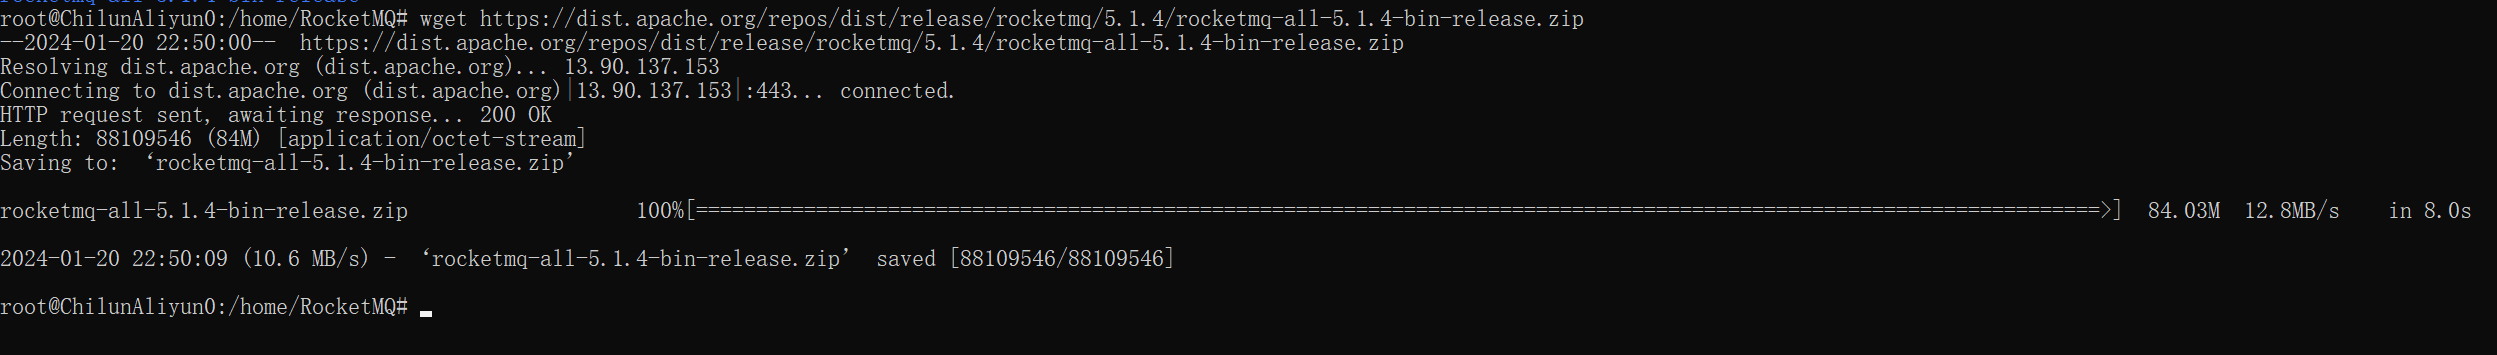
\includegraphics[width=\textwidth]{picture/下载二进制文件.png}
    \captionsetup{hypcap=false}
    \captionof{figure}{下载二进制压缩包}
    \label{fig:下载二进制压缩包}
  \end{minipage}
\end{center}

使用unzip命令解压二进制文件压缩包:\\{\bfseries\kaishu unzip rocketmq-all-5.1.4-bin-release.zip}
\begin{center}
  \begin{minipage}{\textwidth}
    \center
    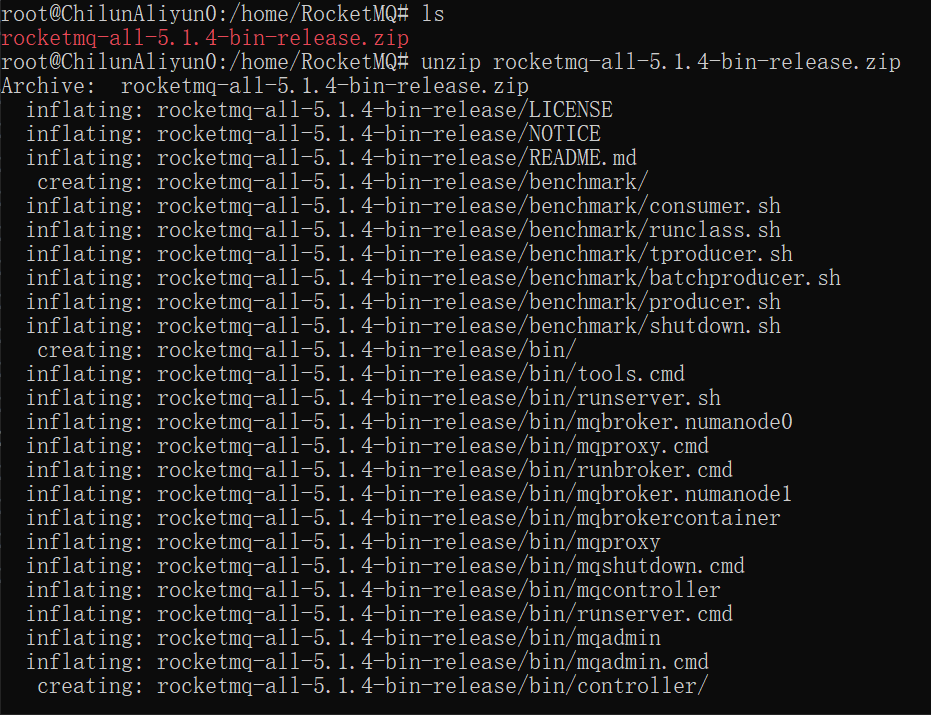
\includegraphics[width=0.7\textwidth]{picture/解压二进制文件.png}
    \captionsetup{hypcap=false}
    \captionof{figure}{解压二进制文件}
    \label{fig:解压二进制文件}
  \end{minipage}
\end{center}

\section{启动NameServer}
进入目录rocketmq-all-5.1.4-bin-release,执行命令:\\{\bfseries\kaishu nohup sh bin/mqnamesrv \&}

命令讲解:
\begin{itemize}
  \item {\bfseries\kaishu nohup:}这代表“不挂起”。在终端中执行命令然后关闭终端时,与该命令相关联的进程通常也会终止。nohup可以防止这种情况发生。
  \item sh:执行脚本文件的shell命令。
  \item bin/mqnamesrv:要运行的脚本路径。
  \item \&:后台运行。
\end{itemize}

发现运行失败:
\begin{center}
  \begin{minipage}{\textwidth}
    \center
    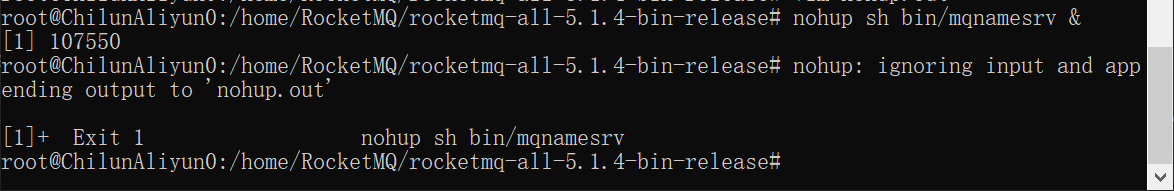
\includegraphics[width=\textwidth]{picture/名字服务器启动失败.png}
    \captionsetup{hypcap=false}
    \captionof{figure}{名字服务器启动失败}
    \label{fig:名字服务器启动失败}
  \end{minipage}
\end{center}

查看nohup.out文件,发现报错:{\bfseries\kaishu OpenJDK 64-Bit Server VM warning: INFO: \\os::commit\_memory(0x0000000700000000, 4294967296, 0) failed; error=\texttt{'}Not enough space\texttt{'} (errno=12)}

操作系统内存不足(由于RocketMQ对内存要求极高,所以自己用云服务器运行基本都会报错),进行修改:

进入rocketmq-all-5.1.4-bin-release/bin目录,对runserver.sh 和 runbroker.sh 以及 tools.sh进行修改。(可使用vim的/+关键字进行查找)
\begin{enumerate}
  \item runserver.sh:
  \\{\bfseries\kaishu JAVA\_OPT=\texttt{"}\${JAVA\_OPT} -server -Xms4g -Xmx4g -Xmn2g -XX:MetaspaceSize=128m 
  \\-XX:MaxMetaspaceSize=320m\texttt{"}}
  \\替换为
  \\{\bfseries\kaishu JAVA\_OPT=\texttt{"}\${JAVA\_OPT} -server -Xms256m -Xmx256m -Xmn128m 
  \\-XX:MetaspaceSize=128m -XX:MaxMetaspaceSize=320m\texttt{"}}
  \\注意有两处。
  \item runbroker.sh:
  \\{\bfseries\kaishu JAVA\_OPT=\texttt{"}\${JAVA\_OPT} -server -Xms8g -Xmx8g\texttt{"}}
  \\替换为{\bfseries\kaishu JAVA\_OPT=\texttt{"}\${JAVA\_OPT} -server -Xms256m -Xmx256m\texttt{"}},
  \\{\bfseries\kaishu JAVA\_OPT=\texttt{"}\${JAVA\_OPT} -Xmn8G -XX:+UseConcMarkSweepGC }
  \\替换为
  \\{\bfseries\kaishu JAVA\_OPT=\texttt{"}\${JAVA\_OPT} -Xmn256m -XX:+UseConcMarkSweepGC }
  \item tools.sh:
  \\{\bfseries\kaishu JAVA\_OPT=\texttt{"}\${JAVA\_OPT} -server -Xms1g -Xmx1g -Xmn256m -XX:MetaspaceSize=128m 
  \\-XX:MaxMetaspaceSize=128m\texttt{"}}
  \\替换为
  \\{\bfseries\kaishu JAVA\_OPT=\texttt{"}\${JAVA\_OPT} -server -Xms256g -Xmx256g -Xmn128m 
  \\-XX:MetaspaceSize=128m -XX:MaxMetaspaceSize=128m\texttt{"}}。
\end{enumerate}

再次输入命令:{\bfseries\kaishu nohup sh bin/mqnamesrv \&}

未报错,查看nohup.out文件,发现启动成功:
\begin{center}
  \begin{minipage}{\textwidth}
    \center
    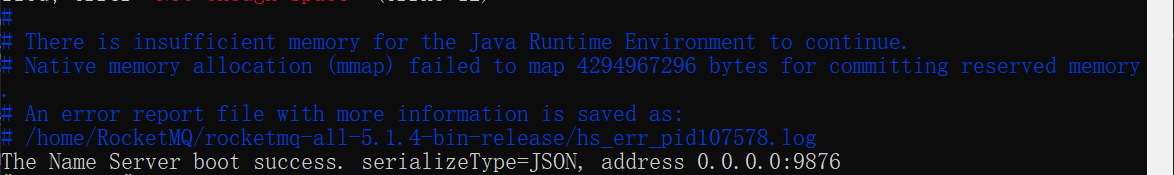
\includegraphics[width=\textwidth]{picture/名称服务器启动成功.png}
    \captionsetup{hypcap=false}
    \captionof{figure}{名称服务器启动成功}
    \label{fig:名称服务器启动成功}
  \end{minipage}
\end{center}

\section{启动Broker+Proxy}
执行命令:\\{\bfseries\kaishu nohup sh bin/mqbroker -n localhost:9876 --enable-proxy \&}

未报错,查看nohup.out文件,发现启动还是失败:
\begin{center}
  \begin{minipage}{\textwidth}
    \center
    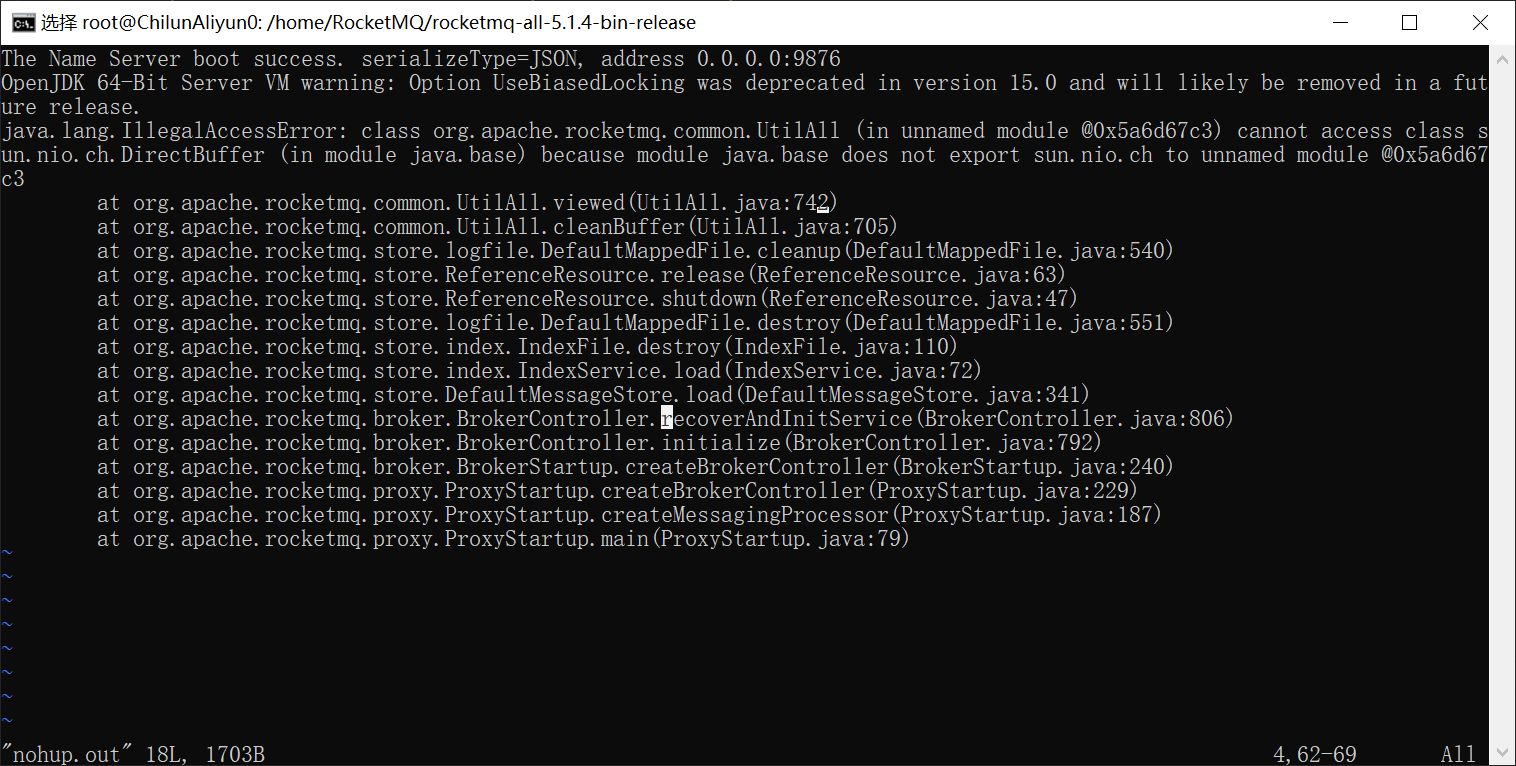
\includegraphics[width=\textwidth]{picture/broker启动失败.png}
    \captionsetup{hypcap=false}
    \captionof{figure}{broker启动失败}
    \label{fig:broker启动失败}
  \end{minipage}
\end{center}

原因是JAVA版本过高,进行修复。

修改runbroker.sh文件:

在{\bfseries\kaishu numactl --interleave=all pwd > /dev/null 2>\&1}上方添加

{\bfseries\kaishu \$JAVA \${JAVA\_OPT} {-}{-}add-exports=java.base/sun.nio.ch=ALL-UNNAMED \$@}


然后再次运行{\bfseries\kaishu nohup sh bin/mqbroker -n localhost:9876 –enable-proxy \&}

并查看nohup.out,发现为不断更新的日志文件,推测运行成功。

查看/root/logs/rocketmqlogs,发现运行成功。
\begin{center}
  \begin{minipage}{\textwidth}
    \center
    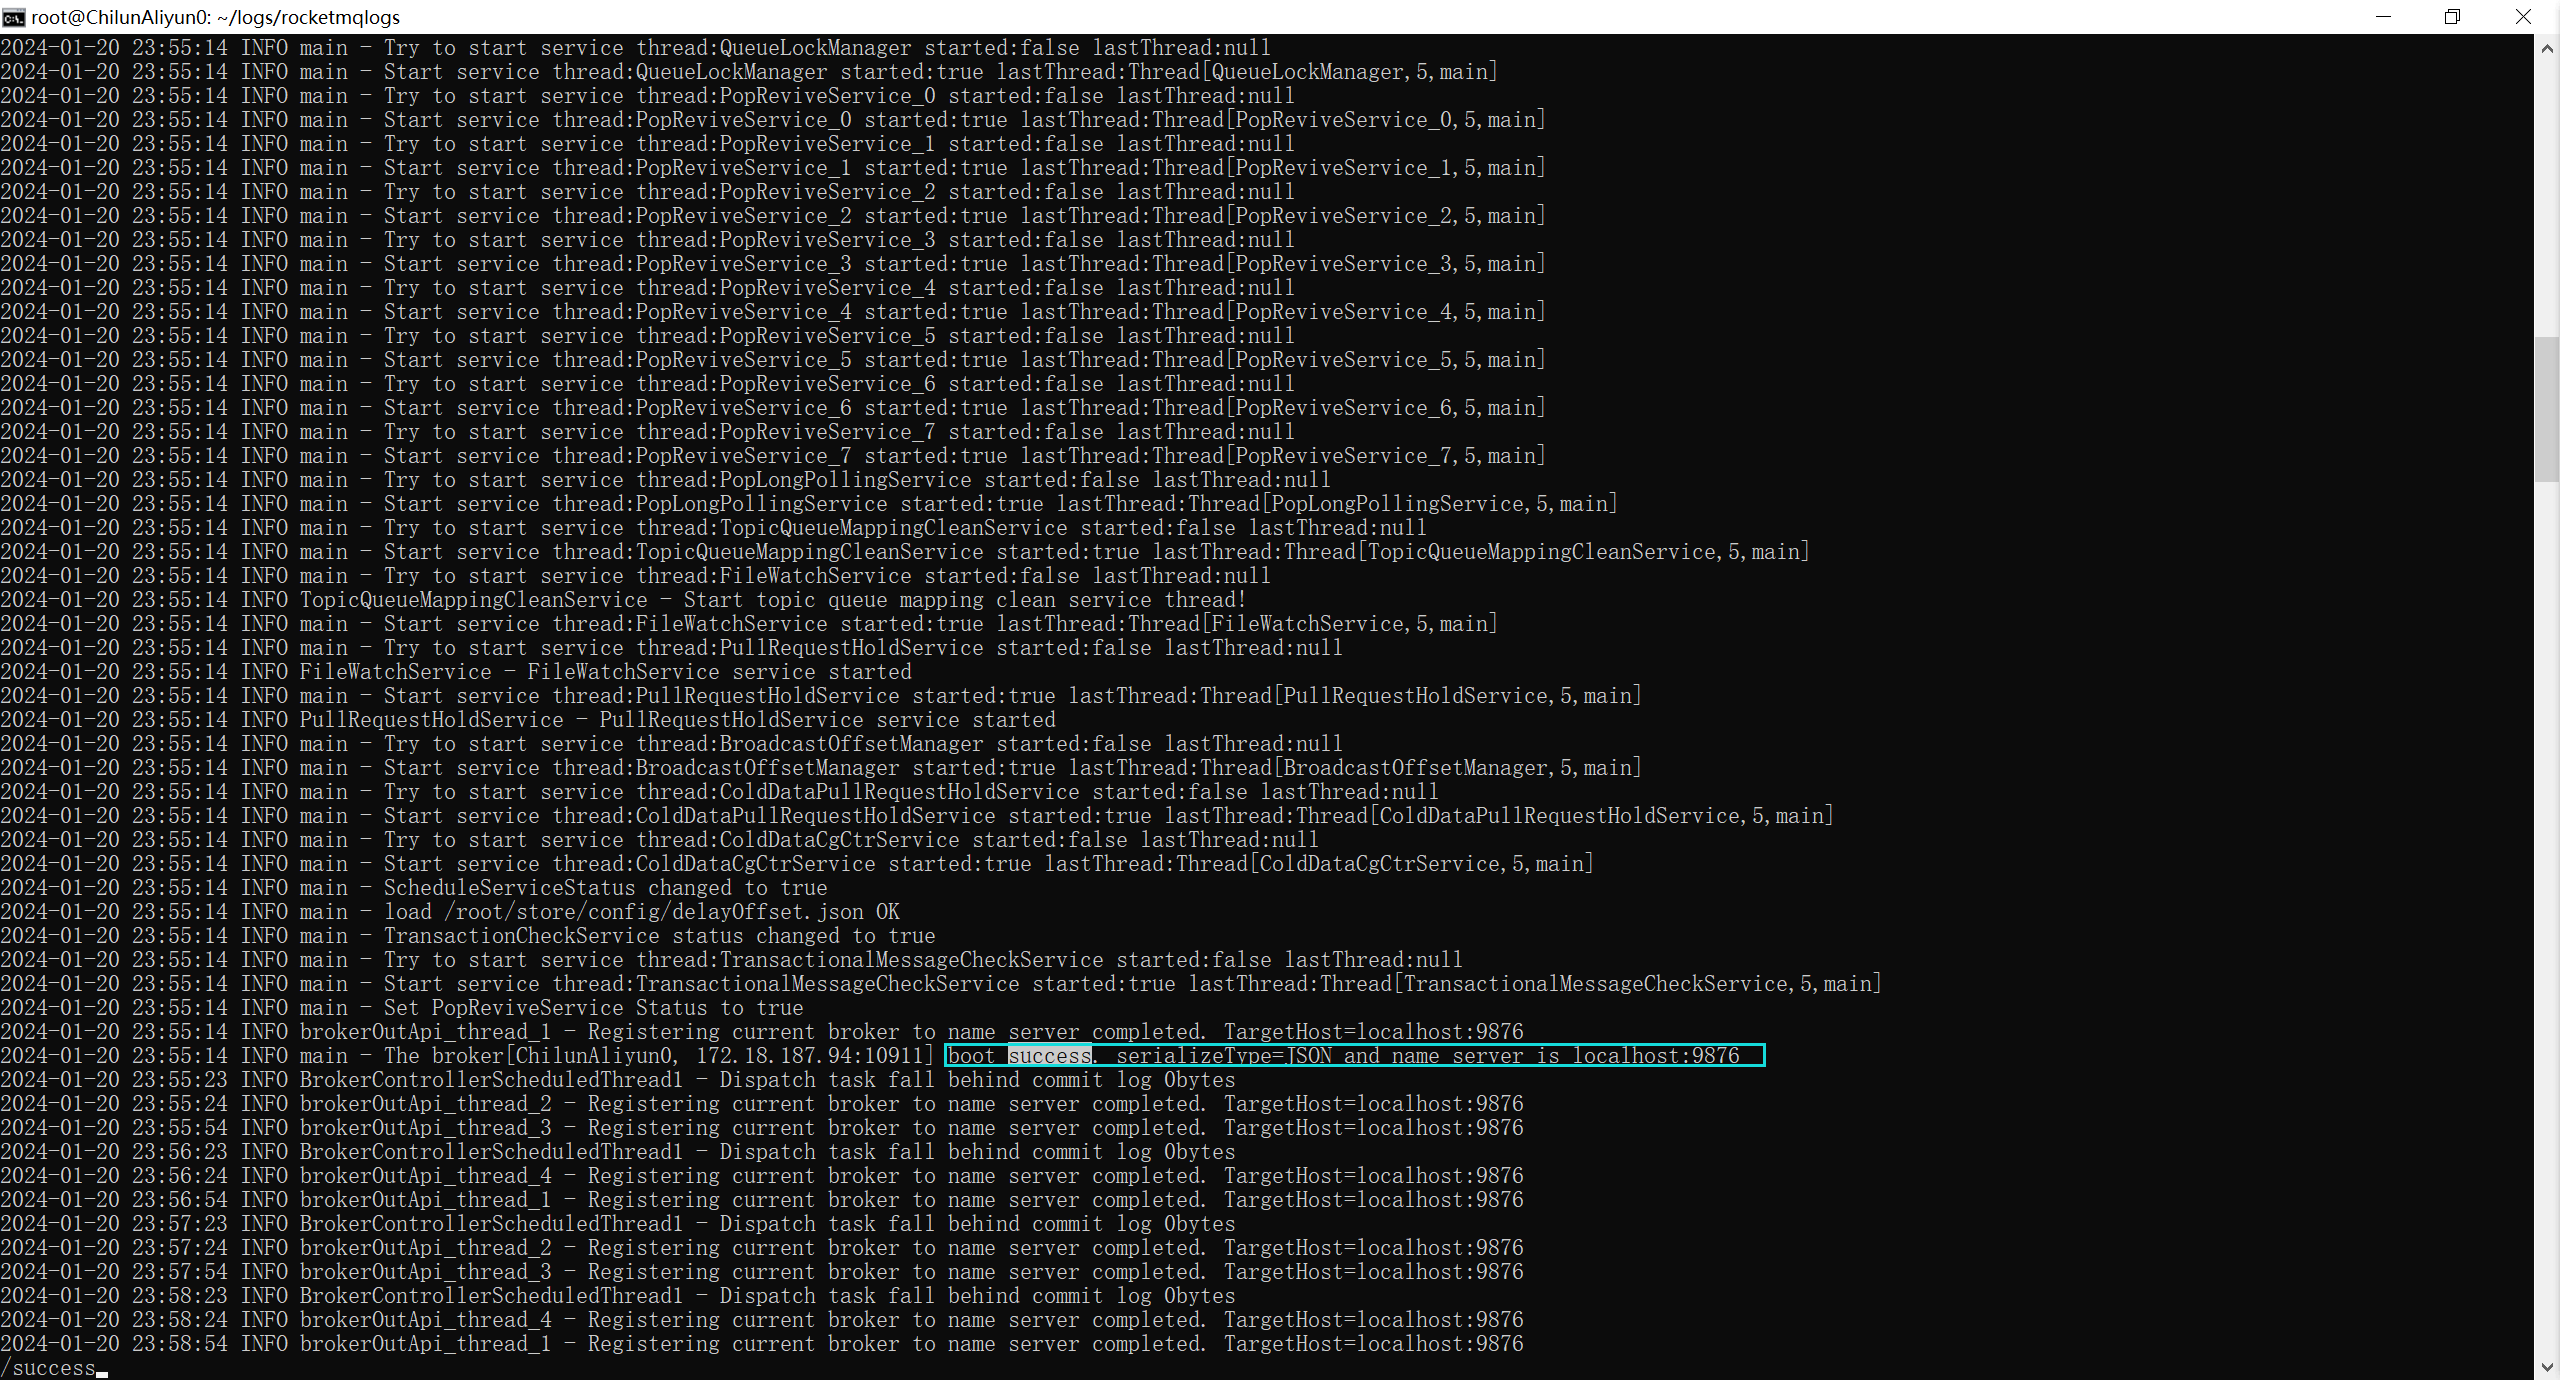
\includegraphics[width=\textwidth]{picture/broker启动成功.png}
    \captionsetup{hypcap=false}
    \captionof{figure}{broker启动成功}
    \label{fig:broker启动成功}
  \end{minipage}
\end{center}

至此,RocketMQ启动成功。

\chapter{领域模型}
\section{架构总览}
组件示意图:
\begin{center}
  \begin{minipage}{\textwidth}
    \center
    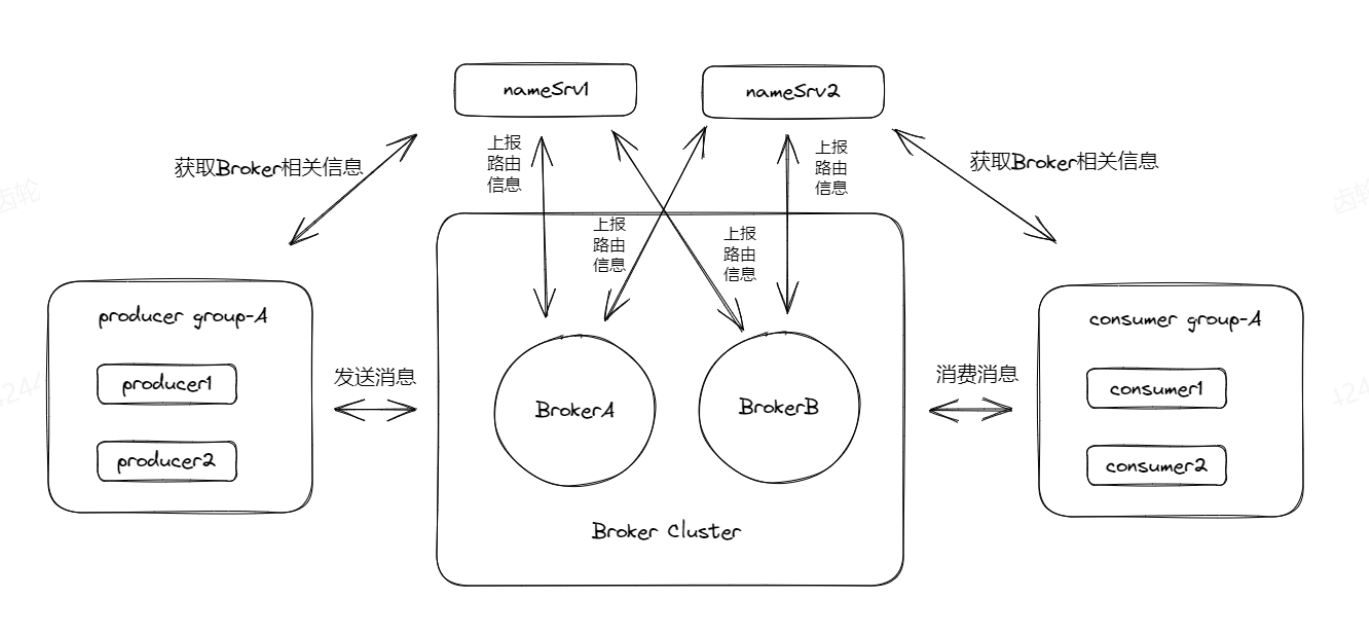
\includegraphics[width=\textwidth]{picture/RocketMQ全局图.jpg}
    \captionsetup{hypcap=false}
    \captionof{figure}{RocketMQ全局图}
    \label{fig:RocketMQ全局图}
  \end{minipage}
\end{center}

\begin{itemize}
  \item {\bfseries\kaishu Producer:}消息生产者。
  \item {\bfseries\kaishu NameSrv:}名称服务,即路由注册中心,可记录中转者提供给消费者和生产者。
  \item {\bfseries\kaishu Broker:}中转者(也可以认为是队列Queen),负责接受、存储、转发消息。
  \item {\bfseries\kaishu Comsumer:}消息消费者。
  \item Producer group:生产者组。
  \item Comsumer group:消费者组。
  \item Broker cluster:中转者集群。
\end{itemize}

\section{基本概念}
领域模型图:
\begin{center}
  \begin{minipage}{\textwidth}
    \center
    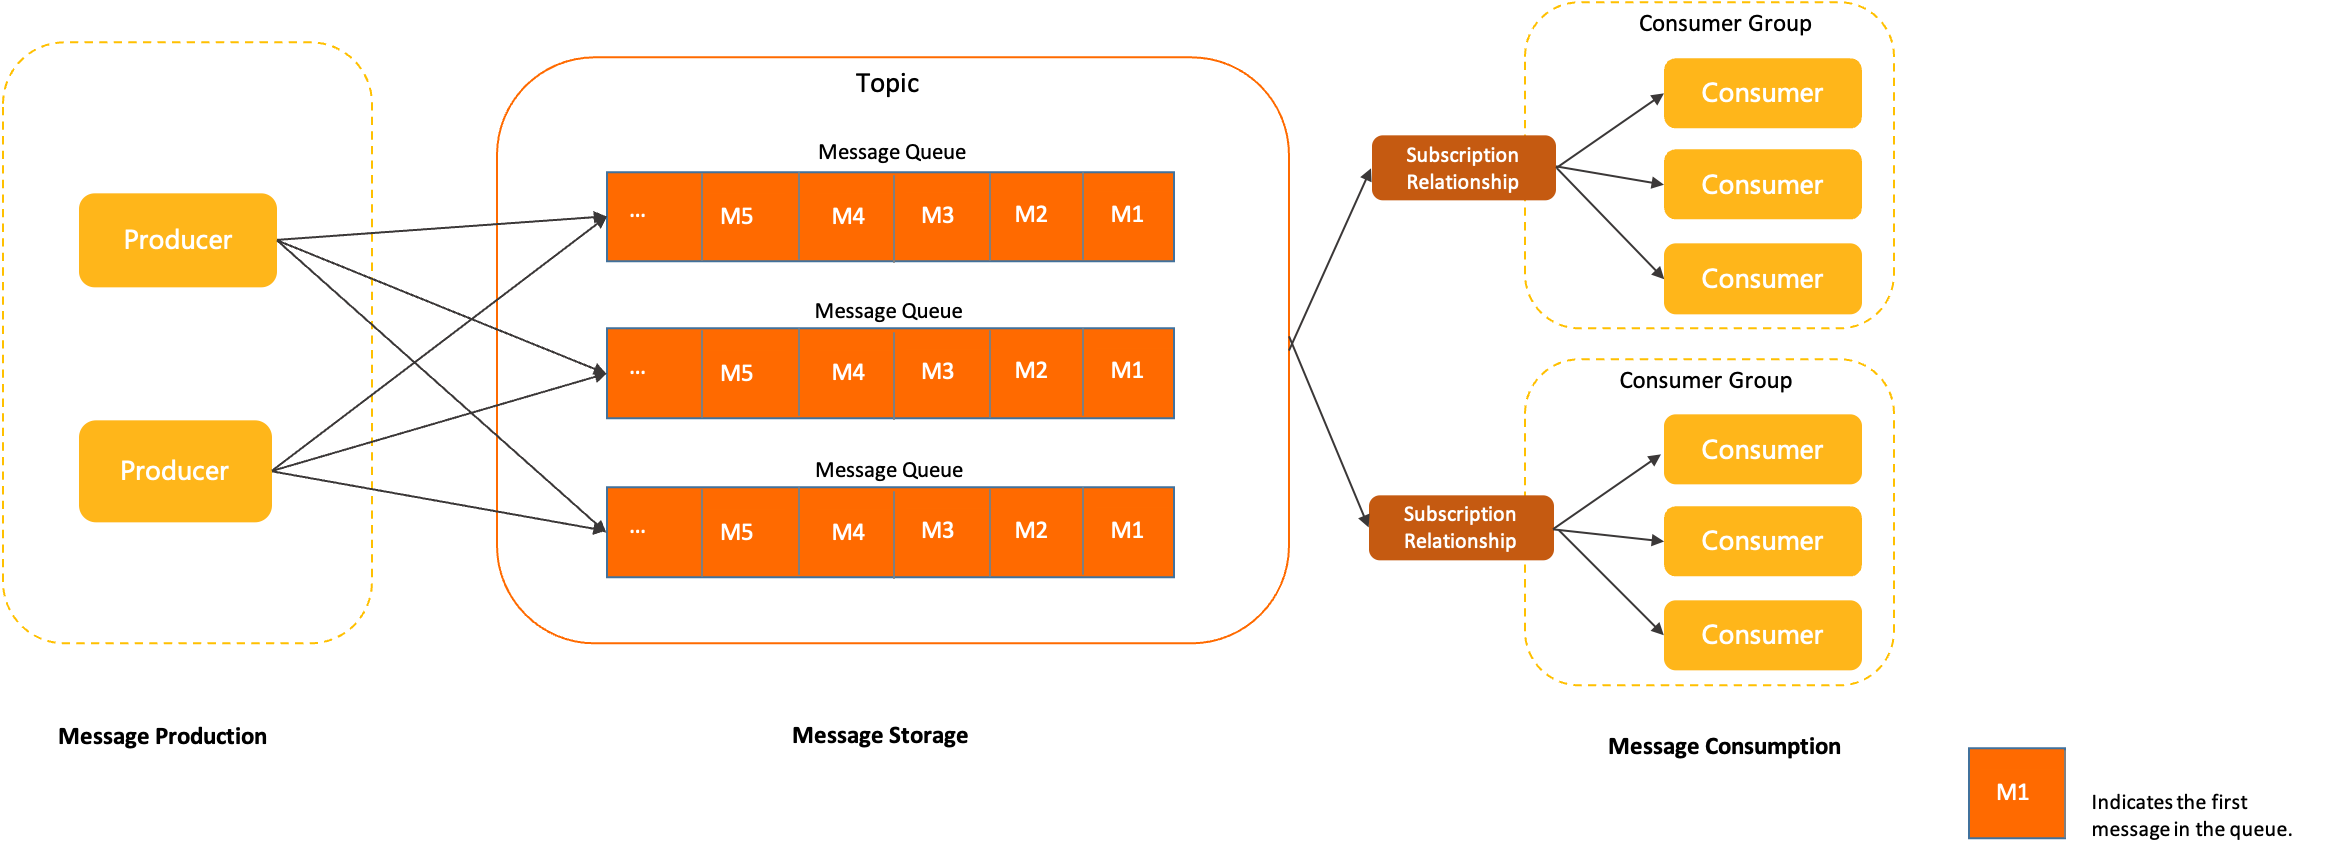
\includegraphics[width=\textwidth]{picture/领域模型图.png}
    \captionsetup{hypcap=false}
    \captionof{figure}{领域模型图}
    \label{fig:领域模型图}
  \end{minipage}
\end{center}

\subsection{消息的生命周期}
RocketMQ 中消息的生命周期主要分为{\bfseries\kaishu 消息生产、消息存储、消息消费}这三部分。

生产者生产消息并发送至RocketMQ 服务端,消息被存储在服务端的主题中,消费者通过订阅主题消费消息。

\subsubsection{消息生产}
\textbf{生产者(Producer):}
在RocketMQ中,生产者是用来发送消息的组件,通常它被集成到业务系统的前端。生产者是轻量级匿名无身份的。

\subsubsection{消息存储}
\textbf{消息(Message):}
RocketMQ 的最小传输单元。消息具备不可变性,在初始化发送和完成存储后即不可变。

\textbf{主题(Topic):}
RocketMQ 消息传输和存储的分组容器,主题内部由多个队列组成,消息的存储和水平扩展实际是通过主题内的队列实现的。

\textbf{队列(MessageQueue):}
RocketMQ 消息传输和存储的实际单元容器,类比于其他消息队列中的分区。 RocketMQ 使用流式特性的无限队列结构来存储消息,消息在队列内会按顺序进行存储。

\subsubsection{消息消费}
\textbf{消费者分组(ConsumerGroup):}
RocketMQ 发布订阅模型中定义的独立的消费身份分组,用于统一管理底层运行的多个消费者(Consumer)。同一个消费组的多个消费者必须保持消费逻辑和配置一致,共同分担该消费组订阅的消息,实现消费能力的水平扩展。

\textbf{消费者(Consumer):}
RocketMQ 消费消息的运行实体,通常它被集成到业务系统的后端。消费者必须被指定到某一个消费组中。

\textbf{订阅关系(Subscription):}
RocketMQ 的订阅关系是指在发布订阅模型中,用于配置消息过滤、重试以及消费进度的规则。订阅关系是以消费组为单位进行管理的,消费组通过定义订阅关系来控制该组下的消费者如何处理消息的过滤、重试以及消费进度恢复等操作。
简单来说,订阅关系就是消费组对消息的一种规则设定,可以让我们更加灵活地控制消息的处理方式,确保系统能够按照我们预期的方式来消费和处理消息。\\
\begin{ignore}
  RocketMQ 的订阅关系除过滤表达式之外都是持久化的,即服务端重启或请求断开,订阅关系依然保留。
\end{ignore}

\subsection{通信方式}
分布式系统架构思想下,将复杂系统拆分为多个独立的子模块,例如微服务模块。此时就需要考虑子模块间的远程通信,典型的通信模式分为以下两种,一种是{\bfseries\kaishu 同步的RPC远程调用};一种是{\bfseries\kaishu 基于中间件代理的异步通信}。

\subsubsection{同步RPC调用模型}
同步RPC调用模型下,不同系统之间直接进行调用通信,每个请求直接从调用方发送到被调用方,然后要求被调用方立即返回响应结果给调用方,以确定本次调用结果是否成功。\\
\begin{ignore}
  注意:此处的同步并不代表RPC的编程接口方式,RPC也可以有异步非阻塞调用的编程方式,但本质上仍然是需要在指定时间内得到目标端的直接响应。
\end{ignore}

\begin{center}
  \begin{minipage}{\textwidth}
    \center
    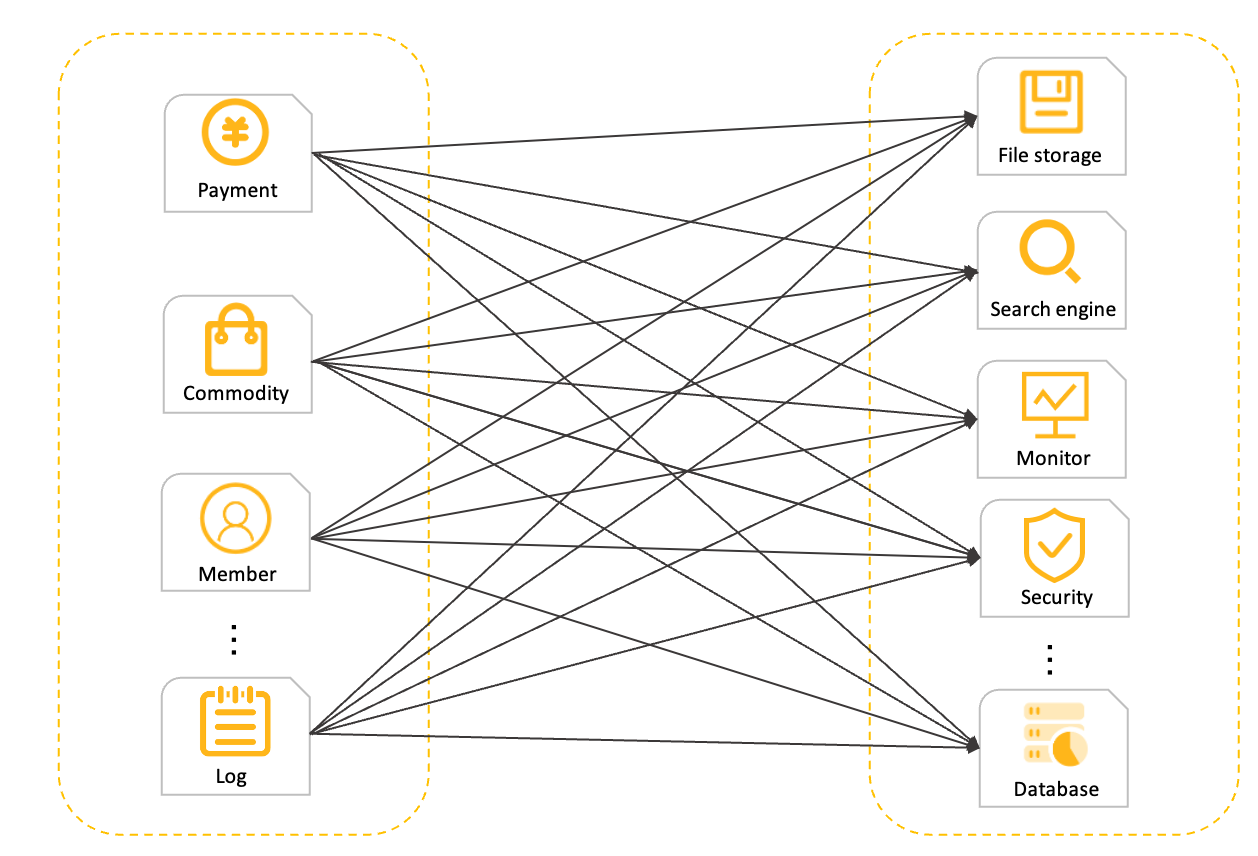
\includegraphics[width=\textwidth]{picture/同步RPC调用模型.png}
    \captionsetup{hypcap=false}
    \captionof{figure}{同步RPC调用模型}
    \label{fig:同步RPC调用模型}
  \end{minipage}
\end{center}

\subsubsection{异步通信模型}
异步消息通信模式下,各子系统之间无需强耦合直接连接,调用方只需要将请求转化成异步事件(消息)发送给中间代理,发送成功即可认为该异步链路调用完成,剩下的工作中间代理会负责将事件可靠通知到下游的调用系统,确保任务执行完成。该中间代理一般就是消息中间件。

\begin{center}
  \begin{minipage}{\textwidth}
    \center
    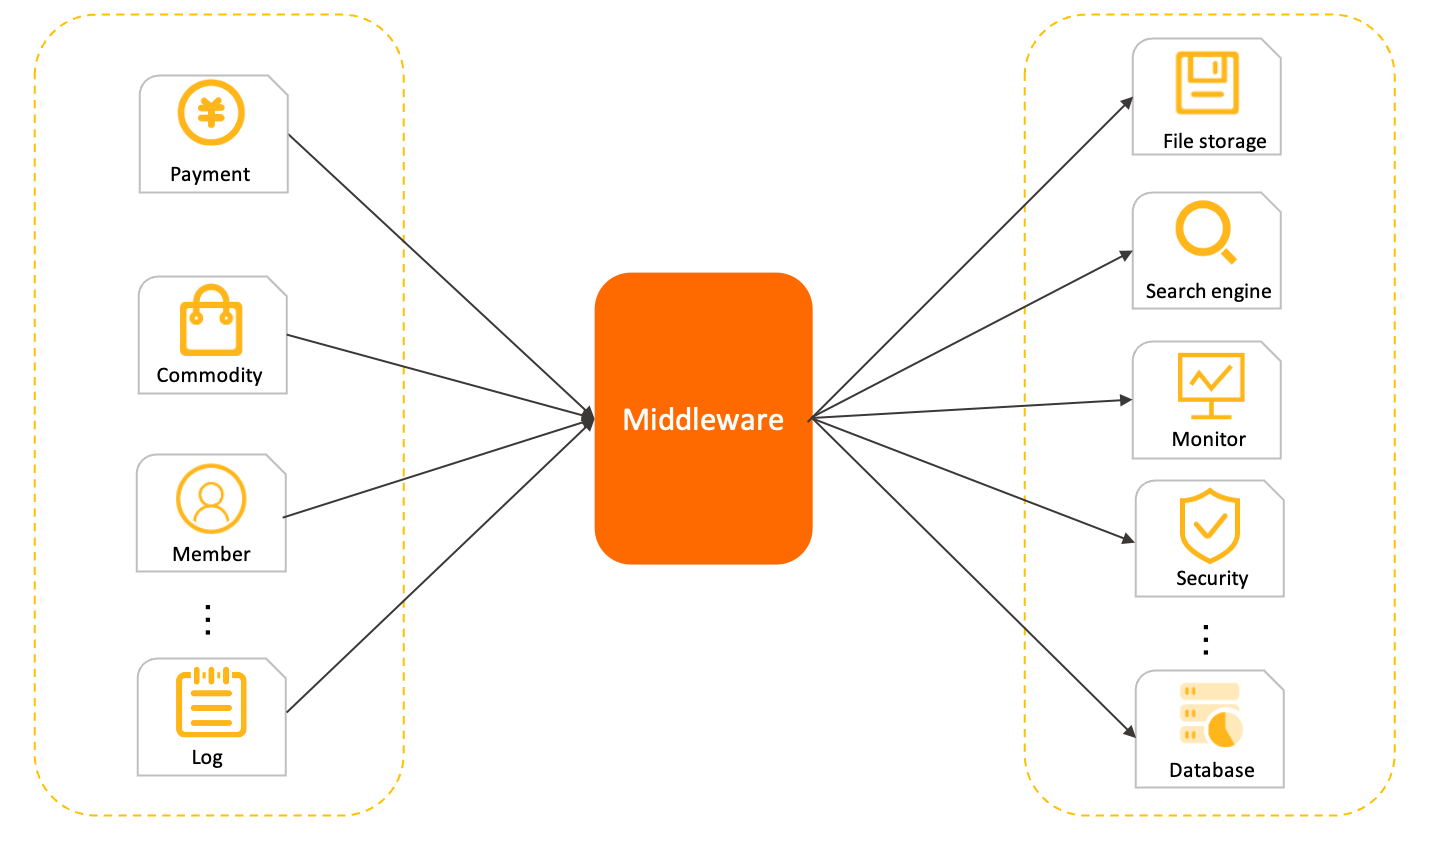
\includegraphics[width=\textwidth]{picture/异步通信模型.png}
    \captionsetup{hypcap=false}
    \captionof{figure}{异步通信模型}
    \label{fig:异步通信模型}
  \end{minipage}
\end{center}

优势如下:
\begin{enumerate}
  \item 星型结构系统,拓扑简单,易于维护和管理。
  \item 上下游耦合性弱,可以独立升级和变更,不会互相影响。
  \item 容量削峰填谷。基于消息的中间代理往往具备很强的流量缓冲和整形能力,业务流量高峰到来时不会击垮下游。
\end{enumerate}




% 文章结束
\end{document}